\par \IEEEPARstart{A}{} continuaci\'on nos explayaremos sobre los detalles de la
implementaci\'on del m\'etodo propuesto. En las secciones previas hemos dado una
introducci\'on al problema, su modelo y justificaci\'on de porque el mismo sirve
y a su vez hemos expuesto un m\'etodo que nos permite hayar la soluci\'on.

\par En esta secci\'on primero hablaremos sobre una implementaci\'on del
algoritmo \ref{alg:power_method2} (p\'agina \pageref{alg:power_method2}), su
justificaci\'on y correctitud. Luego pasaremos a resolver el problema de las
estructuras de datos utilizadas para las matrices del problema (las cuales, por
representar grafos completos, presentar\'an el incoveniente al querer trabajar
con \emph{datasets} cada vez m\'as grandes).

%---------------------------------------------------------------
\subsection{Implementaci\'on del M\'etodo de la Potencia}
\par En la secci\'on previa ya se a presentado dos pseudoc\'odigos (algoritmo
\ref{alg:power_method} y \ref{alg:power_method2}) correspondiente al m\'etodo
que utilizamos durante este trabajo. El principal problema es que ambas opciones
(una siendo una versi\'on simplificada de la otra, para nuestro contexto) es que
computan $x^{(k)} \gets Mx^{(k-1)}$. Recordemos la definici\'on de nuestra
matriz $M$ entonces, de la ecuaci\'on \ref{eq:M}:

\begin{align}
    A &\in\real^{n\times n} / a_{ij} =
        \begin{cases}
            0       &\text{si $j$ no tiene links a $i$}\\
            1/n_j   &\text{si $j$ tiene links a $i$}
        \end{cases}\label{eq:A2}\\
    S &= A + \underbrace{\dfrac{1}{n}e}_{\vec{v}}a^T \quad\quad\quad
        \text{Donde: } a_i =
        \begin{cases}
            1 &\text{si el nodo $i$ es un dangling node}\\
            0 &\text{caso contrario}
        \end{cases}\label{eq:S2}\\
    M &= \alpha S + (1-\alpha)\underbrace{\overbrace{\dfrac{1}{n}e}^{\vec{v}}e^T}_E
    \label{eq:M2}
\end{align}

\par El problema, entonces, es que al computar en cada iteraci\'on $k$ del
m\'etodo de la potencia se efect\'ua la m\'ultiplicaci\'on $Mx^{k-1}$, y $M$ es
una matriz positiva (como ya se a explicado, o como se puede deducir de las
definiciones de las matrices reci\'en expuestas). Entonces tenemos que:

\begin{itemize}
    \item Cada iteraci\'on realizar\'a $2n^2-n$, es decir, $\mathcal{O}(n^2)$
        operaciones matem\'aticas. Cada fila de $M$ multiplca a
        $\vec{x}^{(k-1)}$, realizando $n$ multiplicaciones, para luego sumar
        todos sus resultados ($n-1$ sumas) y obtener una coordenada de
        $\vec{x}^{(k)}$, y esto ocurre para $n$ filas.

    \item Cuando comencemos a trabajar con muchas p\'aginas web, el tama\~no de
        la matriz crecer\'a mucho, y la complejidad espacial de la
        implementaci\'on de la matriz se volver\'a un problema de
        implementaci\'on (ni hablar cuando se trata de
        \emph{rankear}\footnote{Palabra coloquial proveniente del ingl\'es.} a
        todas las p\'aginas de internet).
\end{itemize}
\medskip

\par Kamvar et al. plantean que las aristas \emph{artificiales} introducidas en
la matriz $A$ (que representa el grafo de conectividad pesado seg\'un el grado
de salida de cada nodo) mediante $\vec{v}a^T$ y $E$ no necesitan ser
materializados en la matriz para realizar los c\'aclculos (ya que de antemano
sabemos como afectan a la matriz final $M$ para cualquier operaci\'on que
hagamos con ella)~\cite[p.262]{Kamvar2003}. Por lo tanto, sugieren que el
c\'omputo de $x^{(k)} \gets Mx^{(k-1)}$ sea realizado con el siguiente
algoritmo:

\begin{algorithm}
    \KwIn{vector $\vec{x}^{(k-1)}$; matriz de conectividad pesada $A$; factor de
        navegaci\'on $\alpha$}
    \KwOut{vector $\vec{x^{(k)}}$}
    $\vec{y} \gets \alpha A \vec{x}^{(k-1)}$\;
    $w \gets ||\vec{x}^{(k-1)}||_1 - ||\vec{y}||_1$\;
    $\vec{x}^{(k)}\gets \vec{y}+w\vec{v}$\;
    \KwRet{$\vec{x}^{(k)}$}
    \caption{C\'omputo Eficiente de $x^{(k)}$\cite[p.262]{Kamvar2003}}
    \label{alg:power_method3}
\end{algorithm}

\par En un momento demostraremos que dicho algoritmo es correcto y efectivamente
est\'a computando $Mx^{(k-1)}$. Pero supongamos que asumimos esto como cierto,
¿qu\'e es lo que se gana al implementar de esta manera $Mx^{(k-1)}$?

\begin{wrapfigure}[24]{l}{0.5\textwidth}
    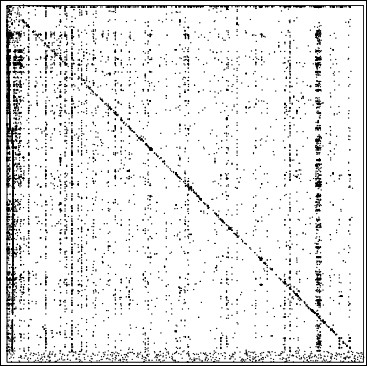
\includegraphics[width=0.48\textwidth]{example6_sparse_google_matrix.jpg}
    \caption{Ejemplo de Matriz Esparsa. Los valores no nulos est\'an indicados
    en negro~\cite[p.34]{Langville2006}}
    \label{fig:sparse_matrix}
\end{wrapfigure}

\par En primer lugar, observemos que nunca se utiliza la matriz $M$, sino que se
usa $A$. Recordemos de la definici\'on de $A$ que la misma es una matriz de
conectividad tal que $a_{ij} = \rfrac{1}{n_j}$ si hay un link de $j$ a $1$ y en
caso contrario sera nulo. Lo interesante a retener, a partir de la definici\'on
de $A$ y algo de conocimiento del dominio del problema, es que para casos muy
grandes la matriz $A$ comienza a ser cada vez m\'as esparsa. Esto ocurre porque
cada p\'agina tiene una cantidad muy acotada de links respecto de la cantidad de
p\'aginas web de internet.

\par En la figura \ref{fig:sparse_matrix} se puede observar un ejemplo real de
una matriz $A$, donde todos los valores son nulos excepto por los pixeles en
negro.

\par As\'i pues, llegamos a computar nuestro $Mx^{(k-1)}$ con una matriz
esparsa. Esto lleva a solucionarnos los 2 problemas planteados de este
c\'omputo. Por un lado las matrices esparsas pueden ser almacenadas utilizando
muy poco espacio en memoria (mediante el uso de estructuras de datos que solo
almacenan los valores no nulos m\'as alguna otra informaci\'on, las cuales
veremos un poco m\'as adelante). Por el otro, la multiplicaci\'on matriz-vector
con una matriz esparsa requiere una complejidad mucho menor que
$\mathcal{O}(n^2)$ operaciones matem\'aticas. De hecho, requiere
$\mathcal{O}(nnz(A))$, para $nnz(A)$ la cantidad de valores no nulos de $A$.
Valores estad\'isticos muestran que la cantidad promedio de links de una
p\'agina web es alrededor de 10, lo que se\~nalar\'ia que $nnz(A)=10n$ en
lugar de los $n^2$ de la matriz $M$~\cite[p.34]{Langville2006}. Entonces pasamos
de tener una complejidad $\mathcal{O}(n^2)$ a $\mathcal{O}(n)$ (por cada fila se
realizan -promedio- 10 multiplicaciones y 9 sumas, obteniendo un costo
$\mathcal{O}(1)$ por fila, para $n$ filas).

\par Claramente, entonces, tendr\'iamos los dos problemas planteados resueltos
en caso de ser equivalentes el c\'omputo de $x^{(k)}\gets Mx^{(k-1)}$ y el
algoritmo \ref{alg:power_method3} propuesto  Luego s\'olo quedar\'ia decidir que
estructura(s) de matrices esparsas utilizar.

%---------------------------------------------------------------
\subsection{Correctitud de C\'omputo de $\mathbf{x^{(k)}\gets Mx^{(k-1)}}$}
\begin{align}
    \intertext{Del algoritmo \ref{alg:power_method3}, reemplazando sus 3 pasos
        principales el uno en el otro, llegamos a que el $x^{(k)}$ devuelto
        ser\'a:}
    &\vec{x}^{(k)} = \alpha A \vec{x}^{(k-1)} + (||\vec{x}^{(k-1)}||_1 - ||\alpha
        A\vec{x}^{(k-1)}||_1)\vec{v}\\
    %
    \intertext{Dado que queremos demostrar que el algoritmo efectivamente
        computa $Mx^{(k-1)}$, lo que queremos demostrar es:}
    &M\vec{x}^{(k-1)} = \alpha A \vec{x}^{(k-1)} + (||\vec{x}^{(k-1)}||_1 -
    ||\alpha A\vec{x}^{(k-1)}||_1)\vec{v}\\
    %
    \intertext{Se puede observar en esto que queremos demostrar, ahora
    s\'olo tenemos $\vec{x}^{(k-1)}$, por lo tanto para facilitar la lectura nos
    referiremos al mismo como $\vec{x}$. Entonces: }
    \text{QVQ: }& M\vec{x} = \alpha A \vec{x} + (||\vec{x}||_1 - ||\alpha
    A\vec{x}||_1)\vec{v}\label{eq:qvq_dem}\\
    %
    \intertext{De las ecuaciones \ref{eq:A2}, \ref{eq:S2} y \ref{eq:M2}, podemos
    llegar a la siguiente definici\'on de $M$:}
    &\begin{aligned}
        M &= \alpha S + (1-\alpha)\vec{v}e^T\\
          &= \alpha(A+\vec{v}a^T)+(1-\alpha)\vec{v}e^T\\
          &= \alpha A+\alpha\vec{v}a^T+\vec{v}e^T-\alpha\vec{v}e^T\\
          &= \alpha A+\vec{v}(e^T-\alpha(e^T-a^T))
    \end{aligned}\\
    %
    \intertext{Luego, multiplicamos por $\vec{x}$}
    &M\vec{x} = \alpha
        A\vec{x} + \vec{v}(\underbrace{e^T\vec{x} - \alpha(e^T\vec{x} -
        a^T\vec{x})}_{\overset{?}{=} ||\vec{x}||_1 - ||\alpha
        A\vec{x}||_1})\label{eq:Mx}\\
    %
    \intertext{Analicemos en primer lugar $e^T\vec{x}$ de esta \'ultima
    ecuaci\'on. Recordemos que $\vec{x}$ era un vector est\'ocastico, entonces:}
    & e^T\vec{x} = \sum_{i=1}^{n}x_i\overarrow[=][\downarrow]{$x_i\geq 0$}
    \sum_{i=1}^{n}|x_i| = ||\vec{x}||_1\label{eq:reemp1}\\
    %
    \intertext{Por otro lado, analicemos $||A\vec{x}||_1$}
    &\begin{aligned}
        ||A\vec{x}||_1 &= \sum_{i=1}^{n} \left|\sum_{j=1}^n a_{ij}x_j\right|
            \overarrow[=][\downarrow]{$a_{ij}\geq 0$\\[-15pt]\tiny$x_j\geq 0$}
                \sum_{i=1}^{n} \sum_{j=1}^n |a_{ij}| |x_j|
            =
                \sum_{j=1}^{n}|x_j| \underbrace{\left(\sum_{i=1}^n|a_{ij}|\right)}_{
                    \underarrow[=][\uparrow]{Columna $j$ de $A$ es\\[-15pt]\tiny
                    estoc\'astica si $n_j\neq 0$\\[-15pt]\tiny
                    Ecuaci\'on \ref{eq:A2}}
                    \begin{cases}
                        0 &\text{Si $n_j = 0$}\\
                        1 &\text{Si $n_j\neq 0$}
                    \end{cases}
                }
            \overarrow[=][\downarrow]{$x_i\geq 0$}
                \sum_{\substack{j=1\\n_j\neq 0}}^n x_j\label{eq:sum1}
    \end{aligned}\\
    %
    \intertext{Y ahora analicemos el t\'ermino restante de la ecuaci\'on
    \ref{eq:Mx}:}
    &e^T\vec{x}-a^T\vec{x}
        = \left(\sum_{i=1}^{n}x_i\right)
            - \left(\sum_{\substack{i=1\\n_i=0}}^n x_i\right)
        = \sum_{\substack{i=1\\n_i\neq 0}}^n x_i\label{eq:sum2}\\
    %
    \intertext{Entonces, si observamos las ecuaciones \ref{eq:sum1} y
    \ref{eq:sum2}, llegamos a que:}
    &e^T\vec{x}-a^T\vec{x} = ||A\vec{x}||_1\label{eq:reemp2}\\
    %
    \intertext{Por \'ultimo, si tomamos las igualdades obtenidas en las
    ecuaciones \ref{eq:reemp1} y \ref{eq:reemp2} y las utilizamos en la
    ecuaci\'on \ref{eq:Mx}, llegamos a que:}
    &\begin{aligned}
        M\vec{x} &=
            \alpha A\vec{x} + \vec{v}(||\vec{x}||_1 - \alpha||A\vec{x}||_1)\\
        \overarrow[\implies][\downarrow]{$\alpha\geq 0$}
        M\vec{x} &=
            \alpha A\vec{x} + (||\vec{x}||_1 - ||\alpha A\vec{x}||_1)\vec{v}
    \end{aligned}
\end{align}

\par Que es, justamente, lo que quer\'iamos demostrar (ecuaci\'on \ref{eq:qvq_dem}).

%---------------------------------------------------------------
\subsection{Estructuras de Datos para Matrices
Esparsas\protect\footnote{T\'ermino coloquial utilizada para referirnos a
matrices poco densas, es decir matrices con muchos valores nulos.}}

\subsubsection{Dictionary of Keys (DoK)}

\subsubsection{Compressed Row Storage (CRS)}
